
%\documentclass[preprint,pra]{revtex4-1}
\documentclass[reprint,pra]{revtex4-1}
\usepackage{amsfonts}
\usepackage{amssymb}
\usepackage{amsmath}
\usepackage{hyperref}
\usepackage{graphicx}% Include figure files
\usepackage{epstopdf}
\usepackage{subfig}
\usepackage{makeidx}
\usepackage[page,toc,title,titletoc]{appendix}



%\usepackage{comment}
%%\includecomment{mycomment}
%\specialcomment{mycommentzhu} {\begingroup\ttfamily\footnotesize}{\endgroup}
%%\excludecomment{mycomment}

%%adding comment, use the next line for disable comment
\newcommand{\mycomment}[1]{\textit{#1}}
%\newcommand{\mycomment}[1]{}

%\newcommand{\vk}{\ensuremath{\mathbf{k}}}
\newcommand{\vK}{\ensuremath{\mathbf{K}}}
\providecommand{\vr}{\ensuremath{\mathbf{r}}}
%\newcommand{\vec}[1]{\ensuremath{\mathbf{#1}}}

\newcommand{\gk}{\ensuremath{{g}(\mathbf{k})}}

\newcommand{\vp}{\ensuremath{\mathbf{p}}}
\newcommand{\gp}{\ensuremath{{g}(\mathbf{p})}}

\newcommand{\vq}{\ensuremath{\mathbf{q}}}

\newcommand{\Fo}{\ensuremath{\mathbf{F_0}}}


\newcommand{\E}{\ensuremath{\mathbf{E}}}
\newcommand{\A}{\ensuremath{\mathbf{A}}}
\newcommand{\J}{\ensuremath{\mathcal{J}}}

\newcommand{\ket}[1]{\ensuremath{\left|#1\right>}}
\newcommand{\bra}[1]{\ensuremath{\left<#1\right|}}

\newcommand{\twoe}{\ensuremath{2\epsilon_\vk-\E_1}}

\newcommand{\nth}[1]{\ensuremath{\frac{1}{#1}}}

\newcommand{\br}[1]{\ensuremath{\left(#1\right)}}
\newcommand{\mbr}[1]{\ensuremath{\left[#1\right]}}
\newcommand{\bbr}[1]{\ensuremath{\left\{#1\right\}}}


\newcommand{\tk}{\ensuremath{\tilde{k}}}

\newcommand{\kp}{\ensuremath{\ket{\Psi}}}

\newcommand{\av}[1]{\ensuremath{\bigl<{#1}\bigr>}}
\newcommand{\avs}[3] {\av{#1{\lvert{#2}\rvert}#3}}
\newcommand{\avv}[2][\nu] {\avs{#1}{#2}{#1}}
\newcommand{\avt}[2]{\av{{#1}|{#2}}}
\newcommand{\avtu}[1]{\av{T_\tau#1}}

\newcommand{\Bop}{\ensuremath{\mathbf{B_0^+}}}
\newcommand{\Bmp}{\ensuremath{\mathbf{B_m^+}}}
\newcommand{\Bnp}{\ensuremath{\mathbf{B_n^+}}}
\newcommand{\Bo}{\ensuremath{\mathbf{B_0}}}
\newcommand{\Bopn}{\ensuremath{\mathbf{{B_0^+}^n}}}
\newcommand{\Bon}{\ensuremath{\mathbf{{B_0}^n}}}


\newcommand{\zmatrix}{\ensuremath{\br{\begin{smallmatrix}0&0\\0&0\end{smallmatrix}}}}
\newcommand{\fmtrx}[4]{\ensuremath{\br{\begin{smallmatrix}#1&#2\\#3&#4\end{smallmatrix}}}}
\newcommand{\smtrx}[6]{\ensuremath{\br{\begin{smallmatrix}#1&#2\\#3&#4\\#5&#6\end{smallmatrix}}}}

\newcommand{\vz}{\ensuremath{v^{\beta\alpha}_{\vk,\vk}}}


\providecommand{\abs}[1]{\ensuremath{\lvert{#1}\rvert}}

\newcommand{\sg}[1][1]{\ensuremath{\sigma_\frac{#1}{2}}}

\newcommand{\rhof}{\ensuremath{\rho(\ef)}}
\newcommand{\omt}{\ensuremath{\tilde{\Omega}}}
\newcommand{\cht}{\ensuremath{\tilde{\chi_0}}}
\newcommand{\Atl}{\ensuremath{\abs{A}^{2l}}}
\newcommand{\ef}{\ensuremath{\epsilon_F}}

\newcommand{\lca}{\ensuremath{\ln\br{1+\frac{\cht}{\alpha}}}}

\newcommand{\com}[2]{\ensuremath{\mbr{#1,#2}}}
\newcommand{\D}{\ensuremath{\mathit{D}}}
\newcommand{\dg}{\ensuremath{\dagger}}
\newcommand{\nG}{\ensuremath{\hat{\mathcal{G}}^{-1}}}

\providecommand{\lvk}{\ensuremath{1/\vk_F}}
\providecommand{\hm}{\ensuremath{\frac{\hbar^2}}{2m}}
\providecommand{\pdiff}[2]{\ensuremath{\frac{\partial{#1}}{\partial{#2}}}}
\providecommand{\dpdiff}[2]{\ensuremath{\frac{\partial^2{#1}}{\partial{{#2}^2}}}}

\providecommand{\H}{\ensuremath{\mathcal{H}}}
\providecommand{\wt}[1]{\widetilde{#1}}

\providecommand{\eef}[1]{Eq. (\ref{#1})}

\providecommand{\sch}{{Schr\"{o}dinger }}

\providecommand{\sgn}{\ensuremath{\text{sgn}}}
\newcommand{\Arctg}{\ensuremath{\text{Arctg}}}

\providecommand{\comm}[1]{\textit{\scriptsize \uwave{(#1)}}}
\newcommand{\vk}{\ensuremath{\mathbf{k}}}
\newcommand{\vK}{\ensuremath{\mathbf{K}}}
\providecommand{\vr}{\ensuremath{\mathbf{r}}}
\newcommand{\vp}{\ensuremath{\mathbf{p}}}
\providecommand{\sch}{{Schr\"{o}dinger }}
\newcommand{\nth}[1]{\ensuremath{\frac{1}{#1}}}

\newcommand{\br}[1]{\ensuremath{\left(#1\right)}}
\newcommand{\mbr}[1]{\ensuremath{\left[#1\right]}}
\newcommand{\bbr}[1]{\ensuremath{\left\{#1\right\}}}
\providecommand{\abs}[1]{\ensuremath{\left\lvert{#1}\right\rvert}}

\newcommand{\fmtrx}[4]{\ensuremath{\br{\begin{smallmatrix}#1&#2\\#3&#4\end{smallmatrix}}}}
\newcommand{\smtrx}[6]{\ensuremath{\br{\begin{smallmatrix}#1&#2\\#3&#4\\#5&#6\end{smallmatrix}}}}
\newcommand{\mtrx}[1]{\ensuremath{\begin{pmatrix}#1\end{pmatrix}}}

\newcommand{\dg}{\ensuremath{\dagger}}
\newcommand{\tr}{\ensuremath{\text{tr}}}
\newcommand{\nG}{\ensuremath{\hat{\mathcal{G}}^{-1}}}

\newcommand{\av}[1]{\ensuremath{\bigl<{#1}\bigr>}}
\newcommand{\avs}[3] {\av{#1{\lvert{#2}\rvert}#3}}
\newcommand{\avv}[2][\nu] {\avs{#1}{#2}{#1}}
\newcommand{\avt}[2]{\av{{#1}|{#2}}}
\newcommand{\avtu}[1]{\av{T_\tau#1}}

%\newenvironment{unsure}
%	{\begin{itshape}}% begin code
%	{\end{itshape}}%                    end code
%\newenvironment{unsure}{}{}



\begin{document}


\title{BEC-BCS Crossover with Feshbach Resonance for a Three-Hyperfine-Species Model}
\author{Guojun Zhu}
\email{gzhu1@illinois.edu}
\affiliation{Department of Physics, University of Illinois at Urbana-Champaign}
\author{Anthony J. Leggett}
\affiliation{Department of Physics, University of Illinois at Urbana-Champaign}
\email{alleggett@illinois.edu}

%
\begin{abstract}
% In a Feshbach resonance, the effective s-wave scattering length grows when one tunes toward the resonance point, and eventually diverges at this point.  There is one characteristic energy scale, $\delta_c$, defined as, in the negative side of the resonance point, the detuning energy at which the weight of the bound state shifts from predominately in the open-channel to predominately in the closed-channel.  When the many-body energy scale (e.g. the Fermi energy, $E_{F}$) is larger than $\delta_c$, the closed-channel weight is significant and has to be included in the many-body theory.  Furthermore, when two channels share a hyperfine species, the Pauli exclusion between fermions from two channels also needs to be taken into consideration in the many-body theory.  
%In a narrow Feshbach resonance,  the closed-channel weight is significant and has to be included directly in the many-body theory.  Furthermore, when two channels share a hyperfine species, the Pauli principle prevents  atoms of both channels from occupying the same momentum level, which has no two-body physics counterpart and therefore requires many-body consideration from the very beginning.  
%In the current paper, a set of gap equations and number equations  are derived at the mean-field level.  The fermionic and bosonic excitation spectra are then also studied. Assuming that the uncoupled bound-state of the closed-channel in resonance is much smaller than the inter-particle distance and  the s-wave scattering length, we find that  the basic equations in the single-channel crossover model are still valid. The correction first comes from the existing of the finite chemical potential and additional counting complication due to the closed-channel.  These two corrections need to be included into the mean-field equations, i.e. the gap equations and the number equations, and to be solved self-consistently.  Then the correction due to the inter-channel Pauli exclusion is in the  order of the ratio of the Fermi energy and the Zeeman energy difference between two channels, $E_F/\eta$, which can be analyzed perturbatively over the previous corrections.  
We consider the behavior of an ultracold Fermi gas across a narrow
Feshbach resonance, where the occupation of the closed channel may not be
negligible. While the corrections to the single-channel formulae associated
with the nonzero chemical potential and with particle conservation have
been considered in the existing literature, there is a further effect which
to the best of our knowledge has until now escaped attention, namely the
``inter-channel Pauli exclusion principle" associated with the fact that
a single hyperfine species may be common to the two channels. We focus on
this effect and show that, as intuitively expected, the resulting
corrections are of order $E_F/\eta$, where $E_F$ is the Fermi energy of the gas
in the absence of interactions and $\eta$ is the Zeeman energy difference
between the two channels. We also consider the related corrections
to the fermionic excitation spectrum, and briefly discuss the collective
modes of the system.
\end{abstract}
\pacs{67.85.Lm}
\maketitle
%% Create a dedication in italics with no heading, centered vertically
%% on the page.


%% Create an Acknowledgements page, many departments require you to
%% include funding support in this.
\section{Introduction}

In a low-temperature dilute system, a short-range interaction can be characterized with a single parameter, $a_s$, a.k.a. the s-wave scattering length.    A very desirable property of the Feshbach resonance in such a system is that the effective interaction is tunable experimentally through the Zeeman energy difference between channels which is in turn  tunable through  instruments such as a magnetic field  \cite{Fano,nuclear,ChinRMP,Pethick}. 
 \begin{equation}
a_{s}(B)=a_{bg}\br{1+\frac{\Delta{B}}{B-B_{0}}}
\end{equation}
where $B_{0}$ is the magnetic field at which the $a_{s}$ diverges, i.e., the  resonant point. 
This unique ability gives physicists a rare opportunity to study  a many-body system under various interaction strengths,  and thus connect different physics originally developed separately.  Particularly for the fermionic gas, there are a series of  theoretical works about uniform treatment of  BEC and BCS since the 1960s \cite{Eagle,LeggettCrossover,Nozieres,RanderiaBEC}, for which the dilute ultracold fermionic alkali gas with  Feshbach resonances provides a perfect testing ground.  Indeed,  these theories work quite well  qualitatively.  

%One important characteristic quantity of Feshbach resonance is $\delta_{C}$N (see detail in Chapter \ref{sec:intro:twobody} for details): when detuning from resonance is smaller than it, open-channel atoms dominate and closed-channel can be neglected.  The effective interaction can still be characterized by $a_{s}$.  One seems to acquire a ``magic knob'' that can tune the interaction between atoms.  On the other hand, when negative tuning is much larger than $\delta_{C}$, atoms in closed-channel have comparable weight to that of open-channel or even dominate them.  Two channels need to be considered at the same time.  


%This paper tries to look into the idiosyncrasy of the Feshbach resonance in contrast with a true ``Simple'' knob of the interaction strength.
\begin{figure}[htbp]
\begin{center}
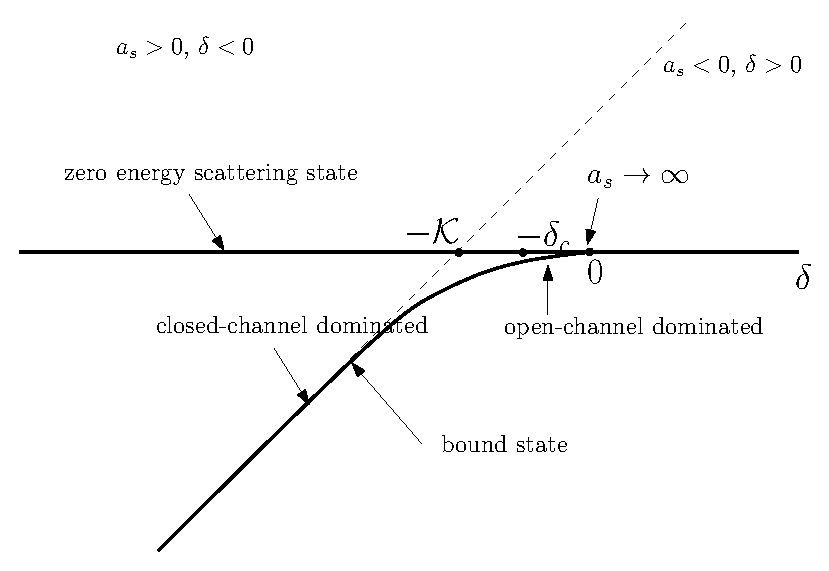
\includegraphics[width=0.8\columnwidth]{levels}
\caption{Energy levels in a Feshbach resonance\label{fig:intro:levels}} 
\parbox{0.9\columnwidth}{\raggedright \small $\delta$ is the energy detuning from the resonance point.  The horizontal line stands for the zero energy s-wave scattering state, $\psi\sim\nth{r}-\nth{a_s}$, which exists for any detuning.  The lower solid line stands for the real bound state, which only exists for negative detuning ($\delta<0$, $a_s>0$). The dashed line stands for the (uncoupled) closed-channel bound state.  An interesting point to notice is that the real bound state appears earlier than the cross point of the (uncoupled) closed-channel bound-state level and zero energy. Another important point to notice is the negative detuning $-\delta_c$.  When the negative detuning is smaller than $\delta_c$, this real bound state is composed mostly with atoms in the open channel and vice versa.  %See Section \ref{sec:model} for details about $\mathcal{K}$ and $\delta_c$.   
}

\end{center}
\end{figure}

  The two-body theory of the Feshbach resonance has a characteristic  parameter, $\delta_c\sim{}a_{bg}^2(\Delta{B})^2$, defined as  the detuning energy at which the weight of the bound state shifts from predominantly in the open channel to predominantly in the closed channel (see Fig. \ref{fig:intro:levels}) \cite{Leggett}.  Na\"{i}vely speaking, on the negative detuning side of any resonance (i.e. $\delta<0$), the two particles should mostly stay  in a (virtual) bound state of the closed channel (or ``virtual state'' in some other-type resonances).  However, at the resonance point  of a Feshbach resonance ($a_s\to\pm\infty$), the atoms are mostly still in the open channel, and they do so down to a negative detuning $\delta\sim-\delta_c$. Only when the negative detuning from resonance is much more  than $\delta_c$, do atoms have the majority weight in the closed channel.    
  
  When considering a many-body system with a Feshbach resonance, an important question is how this energy scale, $\delta_c$, compares to the typical many-body energy scale, namely, the Fermi energy of the free fermionic atoms, $E_F$. In the region not too far away from the resonance ($\abs{\delta}\ll\delta_{c}$), the closed-channel weight is negligible if the Fermi energy is much smaller than $\delta_c$, (i.e., \emph{broad resonance}).  Crossover experiments are usually performed at detuning not too far from the resonance, and hence the closed channel can be safely ignored at the many-body level. Eventually, when the detuning is too far away, $\abs{\delta}\gg\delta_{c}$, the bound state is almost like the    uncoupled closed-channel bound state with a little dressing from the open channel.  
  Nevertheless, such a large detuning in the broad resonance is not very interesting because the  resonance effect is very small and the s-wave scattering length, $a_s$, is close to its background  value then.  
  %We nevertheless do not concern such situations for the broad resonance because crossover phenomena have already be well covered in both BEC and BCS ends with $\abs{\delta}\ll\delta_{c}$. 
 Given the above consideration, for most purposes, we can almost neglect the closed channel  and the problem can be well-described as a two-species fermion system with a tunable interaction when it is not too far away from the resonance.  The Feshbach resonance indeed serves as a simple ``magic'' knob to change the interaction strength.  The original  theories developed on  single-channel models  apply to this case directly.  This is also the situation for two  popular experimental systems (${}^{6}\text{Li}$ atoms at 834G, $^{40}\text{K}$ atoms at 224G).   Many theoretical works have been developed using either the single-channel model or  the two-channel model with the broad resonance assumption (e.g. \cite{Holland01,HoUniversal,Fuchs04}). On the contrary, when the Fermi energy of the free fermionic atoms is  comparable to or even larger than $\delta_c$, the closed channel has to be included at the many-body level even for small detuning. Such a situation, previously considered in some works \cite{GurarieNarrow}, is the focus of the current work.
  
  %Nevertheless, one crucial simplification comes from  the fact  that relevant uncoupled closed-channel bound state is  tightly bound, with spatial extension much smaller than  many-body scales, e.g. the interparticle distance, (but often larger than the potential range).  This fact enable us to treat the Pauli exclusion between two channels perturbatively. It is not necessary to handle all the  fermion species simultaneously, which probably requires quite different techniques  other than those discussed in this paper. 

To complicate the problem  further,   configurations of Feshbach resonances often have one common hyperfine species between the two channels. There are three hyperfine species in the  two channels instead of four species (two for each channel).  Two most common systems (${}^{6}\text{Li}$ at 834G, $^{40}\text{K}$ at 224G) both contain three species of fermions although they are broad resonances.  The Pauli exclusion principle prevents  atoms of both channels from occupying the same momentum level simultaneously because of this common species.  This ``inter-channel Pauli exclusion'' has no counterpart in the two-body physics. This peculiar effect  in many-body crossover problems has  received little theoretical attention up to now.    Nevertheless,   narrow resonances do exist \cite{ChinRMP} and it is not  inconceivable to perform many-body experiments using such resonances.  The central concern of this paper is about these situations. 

Roughly speaking, turning from two-body systems to many-body systems brings three new effects into the original two-body problem.  The first effect is closely associated with the Fermi energy:  For a many-body fermionic system at low temperature, most fermions are inactive; only the fermions close to the Fermi surface participate in the interaction processes. Therefore, the energy often needs to be measured from the Fermi surface instead of from zero as in a two-body situation. 
The second effect relates to counting. Unlike in the single-channel problem, there are two relevant densities in the two-channel problem: the density of atoms in the open channel, $n_{o}$, and the density of atoms in the closed channel, $n_{c}$. When the closed-channel weight is small (broad resonance), it is legitimate to treat the total density as the same as the open-channel density.  However, in the narrow resonance, where the closed-channel weight is not negligible, counting becomes complicated.  Extra care is required to specify which channel quantities such as ``density'' refer to.  These two aspects have been   extensively studied previously \cite{GurarieNarrow}.

The last effect is unique to the three-species problem, where one common species is shared by both channels.  The phase spaces of two channels overlap because of  the common species, which prevents both channels have the occupation in the same momentum level simultaneously. This effect is controlled by the wave-function overlap of the states in the two channels. A rough estimate of this overlap can be made: The uncoupled closed-channel bound state which is in resonance with the open-channel zero energy threshold has  relatively small  spatial extension, $a_c$.  Its binding energy $E_b$ is close to the Zeeman energy difference between two channels, $\eta$.  On the other hand, fermions in the open channel fill the lowest  momentum states up to typically the Fermi energy, $E_F$.  By a simple dimensional argument, the ratio $E_F/\eta$ must control the overlap effect. This effect has  not been addressed in any theoretical work to out knowledge.  How it modifies the many-body picture is the central topic of this paper. 

%We can see this from a slightly alternative aspect using two-fermion molecule gas for the uncoupled closed-channel bound state. We assume that the molecule size is $a_{c}$ and the total number of molecules is $N$.  Assuming further that the bound-state is close to threshold,   the bound-state wave function can then be written as $A/(k^{2}+\kappa^{2})$, where $\hbar^{2}\kappa^{2}/2m=E_{b}$, (see Appendix \ref{sec:pathInt2:short-range}). The prefactor ``$A$'' can be determined  by normalization, $\sum_{k=0}^{1/a_{c}}\abs{\psi}^{2}\sim{}N$. Now  we consider all atoms in a typical many-body scale, e.g. the Fermi energy, $E_{F}$, which is going to overlap with levels occupied in the open-channel. Usually, the Fermi energy is much smaller than the energy scale of the closed-channel bound state, $E_{F}\ll{}E_b$.  The total number of atoms in $[0,E_F]$ is roughly $N\cdot(k_{F}a_{c})^{3}$, which is much smaller than $N$. This means that in the two-channel problem, the low momenta,  ($k\lesssim{}k_F$), are still dominated by the open-channel component even when the total number of atoms in the closed-channel is comparable or higher than the total number  of atoms in the open-channel because atoms in the closed-channel are mostly in  high-momentum states.     

The present paper is divided as follows:
Section \ref{sec:model}  defines the many-body model and introduces the appropriate notation for the 3-species case. Section \ref{sec:mean} lists the mean-field results and renormalization. Section \ref{sec:fermionic} lists the results for the fermionic excitation, and section \ref{sec:bosonic} discusses the bosonic modes. We conclude and discuss our approach in Section \ref{sec:conclusion}.  
 Further details of the calculations may be found in ref. \cite{Zhuthesis}. 
%More specifically, Chapter \ref{sec:intro:one} briefly reviews  dilute ultracold alkali gas.   Section \ref{sec:intro:as} in particular examines the idea of ``universality'', which is one of the central ideas in our treatment of the two-channel model.  Chapter \ref{sec:intro:twobody} goes over the Feshbach resonance in two-body physics and  the concept of  the narrow (broad) resonance is introduced. Chapter \ref{sec:intro:1channel} reviews the single-channel BEC-BCS crossover problem as well as the path-integral approach solving it. This chapter serves as the starting point for the solution of the two-channel model. After these reviews,   Chapter \ref{ch:path2} and Chapter \ref{ch:excitation} present my work on the three-species narrow Feshbach resonance within a many-body path-integral framework, in detail.   Chapter \ref{ch:path2} discusses the mean field result while Chapter \ref{ch:excitation} discusses fermionic and bosonic excitations. An earlier attempt   based on the BCS ansatz  approach in mean-field level is given in Appendix \ref{ch:mean}.  Chapter \ref{ch:conclusion} discusses our procedures and their conclusions.  

\section{Model and notation\label{sec:model}}
We denote the three hyperfine species as $a$, $b$ and $c$, where the open channel contains the pair of species $(a,b)$ and the closed channel contains the pair of species $(a,c)$.  We denote the Grassmann variable for species $i$ by $\psi_i$ and write the  two channels in the notation:
\begin{equation}
(\bar\psi\bar\psi)=\mtrx{\bar\psi_{a}\bar\psi_{b}&\bar\psi_{a}\bar\psi_{c}}
\qquad(\psi\psi)=\mtrx{\psi_{b}\psi_{a}\\\psi_{c}\psi_{a}}
\end{equation}
The two-body interaction can then be written as a ($2\times2$)  hermitian  matrix  $\tilde{U}$ 
\begin{equation}
\tilde{U}\equiv{}\mtrx{U&Y\\Y^{*}&V}
\end{equation}
We can now write the finite-temperature action as 
\begin{multline}\label{eq:pathInt2:actionFermi}
S(\bar\psi,\psi)=\int^{\beta}_{0}d\tau\int{d^{d}r}\\
\mbr{\sum_{j}\bar\psi_{j}(\partial_\tau-\nth{2m}\nabla^{2}-\mu+\eta_{j})\psi_{j}
-(\bar\psi\bar\psi)\tilde{U}(\psi\psi)}
\end{multline}
Here $\eta_{i}$ is the Zeeman energy for hyperfine species $i$. We choose the zero so that $\eta_{a}=\eta_{b}=0$, $\eta_{c}=\eta$.  We  perform the Hubbard-Stratonovich transformation here.   Introduce 2-component  auxiliary fields (order parameters), $(\Delta_{1},\Delta_{2})$, coupled to the fermionic fields as 
\begin{equation}\label{eq:pathInt2:DeltaPhi}
\Delta\longrightarrow\Delta-\tilde{U}(\psi\psi)
\end{equation}
%We can derive the action of $\psi$ and $\Delta$
%\begin{multline}\label{eq:pathInt2:actionMix}
%S_{\tau}(\bar\Delta,\Delta,\bar\psi_{i},\psi_{i})=\int^{\beta}_{0}d\tau\int{d^{d}r}\\
%\Big\{\sum_{j}\bar\psi_{j}(\partial_\tau-\nth{2m}\nabla^{2}-\mu+\eta_{j})\psi_{j}\\
%+[\Delta^{\dg}\tilde{U}^{-1}\Delta-(\bar\psi\bar\psi)\Delta-\bar\Delta{}(\psi\psi)]\Big\}
%\end{multline}
We can introduce  a spinor representation   
\begin{equation}
\bar\Psi=\mtrx{\bar\psi_{a}&\psi_{b}&\psi_{c}}\qquad\Psi=\mtrx{\psi_{a}\\\bar\psi_{b}\\\bar\psi_{c}}
\end{equation}
The action can then be rewritten in a more compact form with respect to $\Psi$ and $\bar\Psi$
\begin{equation}\label{eq:pathInt2:actionMixCompact}
S(\bar\Delta,\Delta,\bar\psi_{i},\psi_{i})=\int^{\beta}_{0}d\tau\int{d^{d}r}
	\mbr{\Delta^{\dg}\tilde{U}^{-1}\Delta-\bar\Psi\mathcal{G}^{-1}\Psi}
\end{equation}
where the fermionic correlation $\mathcal{G}^{-1}$ in the momentum-frequency representation is 
\begin{equation}\label{eq:nG}
\mathcal{G}^{-1}=
\begin{pmatrix}
i\omega_{n}-\xi_{k}&\Delta_{1}&\Delta_{2}\\
\bar\Delta_{1}&i\omega_{n}+\xi_{k}&0\\
\bar\Delta_{2}&0&i\omega_{n}+\xi_{k}+\eta
\end{pmatrix}
\end{equation}
where $\xi_{\vk}=\hbar^{2}k^{2}/2m-\mu$. 
The action in Eq. \ref{eq:pathInt2:actionMixCompact} is  bilinear in the quantities $\Psi$, $\bar\Psi$ and we can formally integrate them out, with the result 
\begin{equation}\label{eq:pathInt2:actionD}
S(\bar{\Delta},\Delta)=\int{dx}\br{\bar{\Delta}\tilde{U}^{-1}\Delta-\tr\ln\nG}
\end{equation}
%Note that at this stage $\Delta(\mathbf{r},\tau)$  is not necessarily homogeneous in space or pseudo-time as in the mean-field result.  


\section{Mean-field result and renormalization\label{sec:mean}}
 Eq. (\ref{eq:nG}) can be inverted to get $G$.   The final mean-field equations are (for simplicity,  both $\Delta_{i}$'s are taken as real.\footnote{\label{foot:pathInt2:real}When $Y$ is not real, $\Delta_{1}$ and $\Delta_{2}$ cannot be both real even at the mean field level.  Nevertheless, we can require one  real, then the other will have a phase just to compensate the phase in $Y$.  The final conclusion can be verified to remain valid.   }) 
  \begin{equation}\label{eq:pathInt2:mf}
\mtrx{\Delta_1\\\Delta_2}=\mtrx{U&Y\\Y^{*}&V}\sum_{\vk}\mtrx{h_{1\vk}\\h_{2\vk}}
\end{equation}
  where $ h_{1\vk}$ and $ h_{2\vk}$ are expectations of the abnormal Green's function.
  \begin{gather}
  h_{1\vk}=\av{\psi_{a,-{\vk}}\psi_{b,+{\vk}}}
  =\Delta_{1}\frac{E_{1\,\vk}+\xi_{\vk}+\eta}{(E_{1\,\vk}+E_{2\,\vk})(E_{1\,\vk}+E_{3\,\vk})}\label{eq:pathInt2:h1}\\
  h_{2\vk}=\av{\psi_{a,-{\vk}}\psi_{c,+{\vk}}}
  =\Delta_{2}\frac{E_{1\,\vk}+\xi_{\vk}}{(E_{1\,\vk}+E_{2\,\vk})(E_{1\,\vk}+E_{3\,\vk})}\label{eq:pathInt2:h2}
  \end{gather}
   where  $E_{i\,\vk}$'s are the eigenvalues of the fermionic correlation Eq. \ref{eq:nG} (see details in Sec. \ref{sec:fermionic}). 
   
   There is one  number equation for each channel,  
\begin{gather*}
\sum_{\omega_{n}, \vk}G_{22}e^{(-i\omega_n\delta_-)}=N_{open}\\
\sum_{\omega_{n},\vk}G_{33}e^{(-i\omega_n\delta_-)}=N_{close}
\end{gather*}
 The Matsubara summation can be performed by the normal trick of multiplying the summand by a Fermi function and deforming the contour \footnote{see sec. 4.2.1 in \cite{Altland}, sec. 25 in \cite{Fetter}}.  For the summation at zero temperature, we just need to consider the positive roots, $E_{1\,\vk}$.  It is straightforward to find 
\begin{gather}
N_{\text{open}}=\sum_{\vk}\frac{(E_{1\,\vk}-\xi_{\vk})(E_{1\,\vk}+\xi_{\vk}+\eta)-\Delta_2^2}{(E_{1\,\vk}+E_{2\,\vk})(E_{1\,\vk}+E_{3\,\vk})}
\label{eq:pathInt2:numOpen}\\
N_{\text{closed}}=\sum_{\vk}\frac{(E_{1\,\vk}-\xi_{\vk})(E_{1\,\vk}+\xi_{\vk})-\Delta_1^2}{(E_{1\,\vk}+E_{2\,\vk})(E_{1\,\vk}+E_{3\,\vk})}
\label{eq:pathInt2:numClose}
\end{gather}
 \subsection{The Bogoliubov canonical transformation and the  fermionic excitation\label{sec:fermionic}}
 The fermionic correlation (Eq. \ref{eq:nG}) can be diagonalized with a (unitary) Bogoliubov canonical transformation.  We  break down the transformation into two steps $T_{\vk}$ and $L_{\vk}$ . 
\begin{equation}\label{eq:pathInt2:B}
B_{\omega_{n},\vk}=L_{\vk}^{\dg}T_{\vk}^{\dg}G_{\omega_{n},\vk}^{-1}T_{\vk}L_{\vk}
\end{equation} 
Here $B_{\vk}$ is the diagonal matrix; $T_{\vk}$ and $L_{\vk}$ are both unitary transformations.  We take $T_{\vk}$ as the canonical transformation at the broad resonance, i.e., when we can ignore the inter-channel Pauli exclusion. 
\begin{equation}\label{eq:pathInt2:T}
T_k=\mtrx{u_k&v_k&0\\-v_k&u_k&0\\0&0&1}
\end{equation}	
where $u_{k}$ and $v_{k}$ are defined in a similar fashion as in the single-channel BCS  problem
\begin{gather}
v_{\vk}^{2}\equiv1-u_{\vk}^{2}\equiv\nth{2}\br{1-\frac{\xi_{\vk}}{E_{\vk}}}\\
E_{\vk}\equiv(\xi_{\vk}^{2}+\Delta_{1}^{2})^{1/2}
\end{gather}
 Note that in the narrow resonance here,  $v_{\vk}^{2}$  does not carry the physical meaning of the occupation number of the (open-channel) atoms, and $E_{\vk}$   does not represent the fermionic excitation spectrum. $T_{\vk}$ can be taken as the direct sum of two parts, the first two rows/columns describe the open-channel excitations, while the third row/column describes the closed-channel ones.  It nevertheless is not sufficient to diagonalize the fermionic correlation in the narrow resonance.  

Introduce a dimensionless scale $\zeta$,
\begin{equation}\label{eq:pathInt2:zetaDef}
\boxed{\zeta=\frac{\Delta_{2}^{2}}{\Delta_{1}\eta}\sim\br{\frac{E_{F}}{E_{b}}}^{1/2}\ll1}
\end{equation}
where $E_{b}$ is the binding energy of the uncoupled closed-channel bound state, $\phi$.
Here both $\Delta_{1}$ and $\Delta_{2}$ are their mean-field (saddle point) values.  
It is not hard to find  the additional unitary transformation $L_{\vk}$ to   first order in $\zeta$ .
\begin{gather}\label{eq:pathInt2:L1}
L_{\vk}\approx{}I+
\mtrx{0&-\frac{\Delta_{1}{}\Delta_{2}{}}{4E^{2}_{\vk}}&u_{\vk}\\
\frac{\Delta_{1}{}\Delta_{2}{}}{4E^{2}_{\vk}}&0&v_{\vk}\\
-u_{\vk}&-v_{\vk}&0
}\frac{\Delta_{2}{}}{\eta}
\equiv{}I+\delta_{k}\\
L^{\dg}_{\vk}=I-\delta_{\vk}\nonumber
\end{gather}
So we finally arrive at the diagonal matrix $B_{\omega_{n},\vk}$ to first order in $\zeta$
\begin{equation}\label{eq:pathInt2:Bapprox}
B_{\omega_{n},\vk}=i\omega_{n}I-
	\begin{pmatrix}E_{1}{}_{\vk}&0&0\\0&-E_{2}{}_{\vk}&0\\0&0&-E_{3}{}_{\vk}\end{pmatrix}
\end{equation}
The eigenvalues of $\nG$  in $B_{\omega_{n},\vk}$ describes the dispersion spectrum of the  fermionic excitations
\begin{align}\label{eq:pathInt2:xiExpand}
E_{1\vk}&\approx{}E_{\vk}+\frac{\Delta_{2}^{2}u_{\vk}^{2}}{\xi_{\vk}+\eta}
\approx{}E_{\vk}+u_{\vk}^{2}\Delta_{1}\zeta\\
E_{2\vk}&\approx{}E_{\vk}-\frac{\Delta_{2}^{2}v_{\vk}^{2}}{\xi_{\vk}+\eta}
\approx{}E_{\vk}-v_{\vk}^{2}\Delta_{1}\zeta\label{eq:pathInt2:xiExpand2}\\
E_{3\vk}&\approx{}\xi_{\vk}+\eta-\frac{\Delta_{2}^{2}}{2(\xi_{\vk}+\eta)}
\approx{}\epsilon_{\vk}+\eta-\frac{\zeta}{2}\Delta_{1}
\label{eq:pathInt2:xiExpand3}
\end{align}
    $E_{1\vk}$ and $E_{2\vk}$ correspond to the traditional Bogoliubov quasi-particle modes; while $E_{3\vk}$ describes the fermionic excitation mostly in the closed channel.  The correction due to the inter-channel Pauli exclusion are all of order $\zeta$.

 
 \subsection{Renormalization of the mean-field equation}
    The summations in the gap equations above (Eq. \ref{eq:pathInt2:mf}) diverge when they are converted into integrals at 3D because of the artificial assumption of contact interactions. 
We can nevertheless remove the singularity in two steps.  First, we notice that the closed-channel bound state is much smaller than the interparticle distance. Therefore the two-body correlation within the closed channel is almost unchanged from its two-body value.  Given this consideration, we project the closed-channel correlation $h_{2\vk}$  onto the two-body  bound-state wave function of the uncoupled closed channel, $\phi$.  Second, the bare interaction in the open channel is replaced with a more physically meaningful quantity, the effective s-wave scattering length, $\tilde{a}_s$, which already incorporates the singularity. We refer to ref. \cite{Zhuthesis} for the details of the calculation.  
 
 First, we project the closed-channel correlation $h_{2\vk}$ into  $\phi_{0}$
\begin{equation}\label{eq:pathInt2:hphi}
h_{2\vk}=\alpha\phi^{}_{0\vk}u_{\vk}^{2}
\end{equation}
This projection is only for the high momentum, for the low momentum, the available phase space for the closed channel is much more limited because the atoms in the open channel center in the low momentum.  More specifically, this restriction is represented by the factor $u_{\vk}^2$.  We come to this conclusion because the closed-channel bound state $\phi$ is much smaller in size than the interparticle distance.  This guarantees that the low momentum states are dominated by the open channel.  
Comparing this equation with the two-body \sch equation for $\phi$, we find
\begin{equation}\label{eq:pathInt2:alpha}
\alpha=\frac{\sum_{\vk\vk'}{\phi_{\vk}^{*}}{Y_{\vk\vk'}}{h_{1\vk'}}}{\br{-E_{b}+\eta-2\mu-\lambda_{1}}}
\end{equation}
where
\begin{equation}\label{eq:pathInt2:lambda1}
\lambda_{1}(\eta)\equiv-\sum_{\vk}{\phi_{\vk}^{*}}{(E_{\vk}-\xi_{\vk})}\phi_{\vk}
	-\sum_{\vk\vk'}{\phi_{\vk}^{*}}{v_{\vk'}^{2}V_{\vk\vk'}}\phi_{\vk'}
\end{equation}

Put all these together into the gap equation of the open channel, we find 
\begin{equation*}
\begin{split}
\Delta_{1\vp}=&\sum_{\vk}\br{U_{\vp\vk}+
	\frac{\sum_{\vk^{'}\vp'} Y_{\vp\vp'}{\phi_{\vp'}}{\phi_{\vk'}^{*}}{Y_{\vk\vk'}}}
		{\br{-E_{b}+\eta-2\mu-\lambda_{1}}}}{{h_{1\vk}}}\\
	&-\frac{\sum_{\vk\vk{'}\vp'} Y_{\vp\vp'}{\phi_{\vp'}}{\phi_{\vk'}^{*}}{Y_{\vk\vk'}}v_{\vp'}^{2}{h_{1\vk}}}
		{\br{-E_{b}+\eta-2\mu-\lambda_{1}}}{}
\end{split}
\end{equation*}
Comparing to the similar equations in the two-body problem, we find the detuning from the resonance here differs from that of the two-body physics by $2\mu+\lambda_1$.  $2\mu$ describes the many-body shift of the starting point from zero to the Fermi surface, while $\lambda_1$ describes the inter-channel Pauli exclusion.  Furthermore, the last term in the r.h.s.  is also unique for the many-body problem.  This term has no singularity for high-momentum because of the extra $v_{\vp'}^2$ term in the integral. 

Now we handle the above equation with  the similar strategy as in the single-channel problem: we integrate out the high-momentum part and replace the bare interaction with the more physically observable effective open-channel $a_s$.  
Multiply both side with $(1+TG)$,  where $T$ is the scattering matrix for the open channel, and $G=(\omega-H_{0})^{-1}$ is the Green's function for a free pair in the open channel.\footnote{Here we use the relation between the scattering $T$-matrix, the free pair Green's function $G=(\omega-H_{0})^{-1}$ and the bare interaction $V=-U_{\text{eff}}$.
\begin{equation*}
T=V+TGV=-(1+TG)U_{\text{eff}}
\end{equation*}
 }
\begin{equation*}
(1+TG)\Delta_{1}=-Th_{1}-\lambda_{2}
\end{equation*}
\begin{equation}\label{eq:pathInt2:lambda2}
\lambda_{2\vp}\equiv\alpha\sum_{\tilde\vp\,\vp'}(1+TG)_{\vp\tilde\vp} Y_{\tilde\vp\vp'}{\phi_{\vp'}}v_{\vp'}^{2}
\end{equation}

Using the zero energy value of the free pair Green's function $G(\omega=0)=(-2\epsilon_{\vk})^{-1}$ and introducing the low-momentum s-wave scattering length with extra shift 
\begin{equation}\label{eq:pathInt2:asKshift}
\tilde{a}_s=a_{\text{bg}}(1+\frac{\mathcal{K}}{\delta-2\mu-\lambda_{1}})
\end{equation}
where $\mathcal{K}=\Delta_{\mu}B$, $\Delta_{\mu}$ is the  effective difference of the pair magnetic moments of two channels. And  $\delta$ is the energy detuning between two channels, we have the renormalized open-channel gap equation
\begin{equation}
\begin{split}\label{eq:pathInt2:gapRenorm}
1=&-\frac{\lambda_{2}}{\Delta_{1}}\\
&-\mbr{\frac{4\pi{\tilde{a}_{s}(\mu,\lambda_{1})}}{m}\sum(\nth{2E_{\vk}}-\nth{2\epsilon_{\vk}}-\frac{\Delta_{2}^{2}\xi_{\vk}}{4(\xi_{\vk}+\eta){E_{\vk}^{3}}})}
	\\
\end{split}	
\end{equation}
Here the two factors $\lambda_1$ and $\lambda_2$, given respectively by Eqs. \eqref{eq:pathInt2:lambda1} and \eqref{eq:pathInt2:lambda2}, as well as the last term in the above equation, describe the inter-channel Pauli exclusion effect. All of them involve overlap integrals between the open-channel wave function and the closed-channel wave function.  (The factor $v_{\vk}^{2}$ or $u_{\vk}^{2}$ describes mostly the open-channel wave function, while $\phi$ describes the closed-channel wave function). The larger the overlap of the two, the larger are $\lambda_1$ and $\lambda_2$.  This has a very intuitive interpretation:  more overlap leads to more severe inter-channel Pauli exclusion, which in turn leads to larger (corrections) terms.  In our model, the open-channel wave function is  spread  over  a large region of  real space, (even on the BEC side, the real bound-state is very loosely bound comparing to the closed-channel bound state), while the closed-channel wave function is very sensitive to the binding energy, $E_{b}(\approx\eta)$.  A closed-channel bound state is more spread out  in real space and has larger overlap with the open-channel wave function,  if it is closer to the threshold, i.e.,  the binding energy  is smaller. Consequently,  the terms $\lambda_1$ and $\lambda_2$ are larger in such cases.                           Nevertheless, $\lambda_1$ is much smaller than the  Fermi energy $E_{F}$, or the other shift, the chemical potential, $2\mu$.  So it is still legitimate to treat this shift as a perturbation.  In addition, it is not hard to see that all these terms are linear in the density.

We can also use the expansion on $E_{i\vk}$ in Eqs. (\ref{eq:pathInt2:xiExpand}-\ref{eq:pathInt2:xiExpand3}) to rewrite the two number equations Eqs. (\ref{eq:pathInt2:numOpen}, \ref{eq:pathInt2:numClose}) to  first order in $\zeta$ 
\begin{gather}\label{eq:pathInt2:closeD2}
N_{\text{closed}}\approx\sum_{\vk}\frac{\Delta_{2}^2}{(\xi_{\vk}+\eta)(2\xi_{\vk}+\eta)}
\end{gather}
\begin{equation}
\begin{split}
N_{open}\approx\sum_\vk\mbr{\frac{E_\vk-\xi_\vk}{2E_\vk}(1+\frac{\Delta_{1}}{\eta}\zeta)-\frac{\Delta_{1}^{3}}{4E_\vk^{3}}\zeta
	}	
\end{split}
\end{equation}



%
%
%    In  summary,  the effect of the inter-channel Pauli exclusion is controlled by the small parameter $\zeta$.  The order parameter for the closed-channel can be determined by the number equation of the closed-channel
%\begin{equation}
%N_{close}\approx\sum_{\vk}\frac{\Delta_{2}^2}{(\xi_{\vk}+\eta)(2\xi_{\vk}+\eta)}
%\end{equation}
%The renormalized gap equation is given as
% \begin{equation}
%1=\frac{4\pi{\tilde{a}_{s}(\mu,\lambda_{1})}}{m}\sum(\nth{2E_{\vk}}-\nth{2\epsilon_{\vk}}-\frac{\Delta_{2}^{2}\xi_{\vk}}{4(\xi_{\vk}+\eta){E_{\vk}^{3}}})
%	-\frac{\lambda_{2}}{\Delta_{1}}
%\end{equation}% Here, $\tilde{a}_{s}r(\mu,\lambda_{1})$ is the two-body open-channel effective  s-wave scattering length with  an additional shifting $2\mu+\lambda_{1}$ as
%\begin{equation}
%{a}_{s}=a_{\text{bg}}(1+\frac{\mathcal{K}}{\delta-2\mu-\lambda_{1}})
%\end{equation}
%  $\lambda_{1}$ and $\lambda_{2}$ are two new parameters describing the overlapping of the two channels, and they can be calibrated from  experiments.  The open-channel number equation is
%\begin{equation}
%\begin{split}
%N_{open}\approx\sum_\vk\mbr{\frac{E_\vk-\xi_\vk}{2E_\vk}(1+\frac{\Delta_{1}}{\eta}\zeta)-\frac{\Delta_{1}^{3}}{4E_\vk^{3}}\zeta
%	}	
%\end{split}
%\end{equation}
%The open-channel number equation and the associated gap equation need to be solved self-consistently to get  the mean field result ($\Delta_{1}$ and $\mu$).  One of the most noteworthy new phenomena is probably that the open-channel gap $\Delta_{1}$ saturates in the BEC side of  a narrow resonance. 
%
%  
%  
%  
%  
%
\subsection{Discussion of the mean-field solution\label{sec:pathInt2:mean2}}
As discussed before, the correction of the narrow Feshbach resonance can be taken into account in two steps.  First,  omitting the inter-channel Pauli exclusion, we only consider the chemical potential $\mu$ in the shift and  the extra counting due to the closed channel.  Then in the second step, we can correct the previous result with quantities originated from the inter-channel Pauli-exclusion unique to the three-species problem. 

In  the first step, the gap equation and the (open-channel) number equation are simplified to 
\begin{gather}
1=-\mbr{\frac{4\pi{\tilde{a}_{s}(\mu)}}{m}\sum(\nth{2E_{\vk}}-\nth{2\epsilon_{\vk}})}\label{eq:pathInt2:narrowGapS}\\
N_{\text{open}}=\sum_\vk\frac{E_\vk-\xi_\vk}{2E_\vk}\label{eq:pathInt2:narrowNumS}
\end{gather}
Here we only consider the shift of the  chemical potential $2\mu$ in   $\tilde{a}_s$ (Eq. \ref{eq:pathInt2:asKshift}),
\begin{equation}
\tilde{a}_{s}=a_{\text{bg}}(1+\frac{\mathcal{K}}{\delta-2\mu})\approx{}\frac{a_{\text{bg}}\mathcal{K}}{\delta-2\mu}
%=\frac{\sqrt{2\delta_{c}\hbar^{2}/m}}{\delta-2\mu}
\label{eq:pathInt2:simplenarrowAs}
\end{equation}
The above equations need to be solved self-consistently. 

 An interesting point  to notice is that the gap $\Delta_1$ saturates in the BEC side. This is because the effective attraction in the open channel where the pairing happens is limited by the real attractive strength in the closed channel.  It can not become  infinitely strong as in an ideal single-channel model.  Mathematically, this can be seen from the gap equation, Eqs. (\ref{eq:pathInt2:mf}-\ref{eq:pathInt2:h2}). The closed-channel correlation is limited by the total density, and therefore the gap has a maximum.  

Once this step is finished, we can look for the correction due to the inter-channel Pauli exclusion.  Both $\lambda_1$ and $\lambda_2$ can be shown  to be linear with the density, so can be calibrated by experiments of different densities.  With the proper value of these two parameters, we can find the correction numerically.  It is nevertheless not hard to show that the correction is of order $\zeta$, so that we are warranted to  treat this effect as a perturbation. 


\section{Beyond mean-field:  collective modes\label{sec:bosonic}}
The order parameters ($\Delta_{1}$, $\Delta_{2}$) are defined in terms of the collective behaviors of many fermion atoms.  Fluctuations of the order parameters thus signal the collective excitation modes of the system. Here with a two-component order parameter, four independent modes exist:   two for the magnitude variation of each $\Delta_i$, the internal phase between two $\Delta_i$, and the overall local phase $\theta(x)$ of $\Delta_1$ and $\Delta_2$.  The first three change the magnitude of the action and therefore are massive; while the last one leaves the action invariant and thus is massless. 
We proceed to study two modes of the phase fluctuation.  

The in-sync phase mode is the counterpart of the Anderson-Bogoliubov modes in the single-channel problem. The action $S(\bar{\Delta}_i,\Delta_i)$ (Eq. \ref{eq:pathInt2:actionD}), is invariant if the phases of $\Delta_{1\,\vk}$ and $\Delta_{2\,\vk}$ rotate simultaneously. We therefore conclude that there exists a massless (Goldstone) mode corresponding to the local phase invariance.  Introduce the phase fluctuation $\theta$, 
\begin{equation*}
\Delta_{i}(x)\rightarrow{}\Delta_{i}e^{i2\theta(x)}\qquad{}
\bar{\Delta}_{i}(x)\rightarrow{}\bar{\Delta}_{i}e^{-i2\theta(x)}
\end{equation*}
We have a new action for the phase fluctuation $\theta$
\begin{equation}
S[\theta]=\int{dx}\sum_{q}\theta(q)\theta(-q)\big[\nth{2}\pi^{(0)}(0)\omega_m^2-\frac{n}{2m}q^2\big]
\end{equation}
The fluctuation has a linear dispersion relation and therefore is a sound-like mode.    It is not hard to show that the velocity follows the same structure as that for the single-channel crossover problem \cite{RanderiaBEC} with a correction of order  $\zeta$.

The out-of-sync phase mode can be studied with the similar approach. However, for this mode, we can show that the action is 
\begin{equation}\label{eq:pathInt2:outofphase}
S[\theta]=\int{dx}\sum_{q}\theta(q)\theta(-q)\big[\nth{4}\pi^{(0)}(0)(\omega_m^2-\omega_{0}^{2})-\frac{n}{4m}q^2\big]
\end{equation}
where $\omega_{m}$ has a finite value $\omega_{0}$ at the zero momentum, which indicates a gapped mode. It can be shown that $\omega_{0}$
 is in the order of the ionization (pair breaking) energy, which is around $\Delta_1$ on the BCS side, while around $\abs{\mu}$ on the BEC side. 

\section{Conclusion  and discussion\label{sec:conclusion}}
In this paper, we have studied the narrow Feshbach resonance in  the three-species case where two channels share the same species.  

In general, for the narrow resonance without a shared species, the main correction to the single-channel result comes from the  extra counting of the atoms in the open channel, which leads to the extra shift $2\mu$ in $\tilde{a}_{s}$, and the closed channel, which leads to the extra number equation.  Two number equations exist, one for each channel.  The open-channel number equation resembles the number equation of the single-channel model.

When there is a common species,  however, the  Pauli exclusion between two channels due to the common species in the three-species narrow resonance, calls for careful  consideration. 

  Our treatment follows the the  idea of ``universality'' \cite{Tan2008-1,shizhongUniv}.  For a dilute system with a short-range potential, such as the dilute ultracold alkali gas, the short-range part of a two-body correlation does not significantly change from two-body  to many-body.  This particular feature justifies using the two-body quantities  as the boundary condition for the many-body correlations.  In non-resonant situations, the s-wave scattering length, $a_s$, is a good candidate for such a purpose.  However, in a Feshbach resonance, the open-channel scattering length becomes enormous, comparable to or even larger than the many-body length scale; furthermore, its value is very sensitive to the ratio of weights of atoms in the two channels.  Therefore it is no longer suitable as the two-body characteristic quantity used in  the many-body problem. A better candidate of two-body quantities as boundary condition here is the short-range part of the two-body wave function itself.  In other word, we expect the two-body correlation of the many-body system matches the shape of the two-body wave function  at short distances.  
  
%    The most part of the correlations, where no two particles are close in short-range, is essentially free from interaction. This long-range part of the correlations does change from two-body to many-body.  Unique in our problem is the involvement of the Feshbach resonance.  A resonance makes the system extremely sensitive to even a small change in the relative weight between two channels. We use the fact that,  in the Feshbach resonance, the closed-channel bound state, $\phi_{0}$, as a short-range object,  is still not very sensitive to the resonance; hence, we can, within the universality idea,  apply a simple boundary condition to the closed-channel correlation. However, the indirect interaction mediated by the closed-channel dominates the direct interaction within the open-channel. Consequently, a small change in the closed-channel bound-state weight \emph{does} affect the short-range wave function in the open-channel, originally expressed through the boundary condition using the s-wave scattering length $a_{s}$. 
   %Our treatment follows the spirit of the so-called ``universality'' idea\cite{Tan2008-1,shizhongUniv}.  For a dilute system with a short-range potential, such as the dilute ultracold alkali gas, the short-range part of a two-body correlation does not significantly change from two-body  to many-body.  This particular feature justifies using the two-body quantities (e.g. the s-wave scattering length $a_{s}$) as the boundary condition for the many-body correlations.  The most part of the correlations, where no two particles are close in short-range, is essentially free from interaction. This long-range part of the correlations does change from two-body to many-body.  Unique in our problem is the involvement of the Feshbach resonance.  A resonance makes the system extremely sensitive to even a small change in the relative weight between two channels. We use the fact that,  in the Feshbach resonance, the closed-channel bound state, $\phi_{0}$, as a short-range object,  is still not very sensitive to the resonance; hence, we can, within the universality idea,  apply a simple boundary condition to the closed-channel correlation. However, the indirect interaction mediated by the closed-channel dominates the direct interaction within the open-channel. Consequently, a small change in the closed-channel bound-state weight \emph{does} affect the short-range wave function in the open-channel, originally expressed through the boundary condition using the s-wave scattering length $a_{s}$. 

When the spatial extension $a_c$ of  the closed-channel bound state is  of the order of the   inter-particle distance, $a_{0}$, or even larger, the Feshbach resonance in the many-body context is a genuine three-species many-body problem and no simple solution is available.  By contrast, when the bound-state's spatial extension is much smaller than the interparticle distance, the two-body correlation in the closed channel, which is expected to almost entirely concentrated in the short-range part,  is proportional to  the two-body bound-state wave function. The ratio of the the bound-state size and the interparticle distance, $a_{c}/a_{0}$, serves as the expansion parameter and we can extract  the effect of the inter-channel Pauli exclusion perturbatively.  In essence, we can then  ignore the many-body effects within  closed-channel bound states, while only taking into consideration  the Pauli exclusion between channels and within the open channels.  A few new parameters need to be introduced and can be calibrated from experiments, such as $\lambda_{1}$, $\lambda_{2}$.  Mean field properties can still be determined through gap equations and number equations similarly to the single-channel case.  The excitation modes are also close to the original single-channel result with correction of the order of $\zeta$.
%We can distinguish three different regimes for the many-body energy scale $E_F$ when compared with the two-body physics.  
%\begin{enumerate}
%\item The regime where $E_F$ is much smaller than the characteristic energy $\delta_c$ (See Eq. \ref{eq:intro:deltaC} in Sec. \ref{sec:intro:twobody}). Around resonance, the closed-channel weight is negligible in this regime. We can then ignore the closed-channel completely and approximate the effective open-channel interaction by a  pseudo-potential characterized by the s-wave scattering length, $a_s$. 
%\item The regime where  $E_F$ is larger than $\delta_c$, but smaller than the closed-channel bound state binding energy $E_b$, or the bare detuning $\eta$.  The closed-channel weight is significant in this regime and cannot be ignored, which means $n_{\text{open}}+n_{\text{close}}=n_{\text{total}}$. Also, we need to take into account the fact that, in the resonance formula of $a_s$, shifting should be counted from the Fermi surface instead of from zero as in two-body physics.    These effects, considered previously\cite{GurarieNarrow}, are  also carefully analyzed in this thesis.  Furthermore, the Pauli exclusion between two channels needs to be taken into account when these two channels share a common species.  Nevertheless, at  low momentum, where the open-channel has most of its weight, the closed-channel bound state only has very small weight.  Consequently, we can still treat the Pauli exclusion between channels perturbatively using the expansion coefficient  $E_F/\eta$. 
%\item The regime where  $E_F$ is larger than the binding energy $E_b$ or the bare detuning $\eta$. We have a genuine three-species many-body problem. This regime can be achieved in two ways.  One way requires a very large $E_F$, which indicates a very dense system.  However, it would be hard to imagine that  the original dilute alkali gas model still applies in this case. Various approximations in the model would probably break down beforehand, such as the pseudo-potential approximation with $a_s$. The second way requires a very small $\eta$, which indicates a genuine three-species many-body problem.  This remains an open problem.   
%\end{enumerate}


     In our approach, we take the broad resonance result (or the single-channel crossover) as our zeroth order solution, upon which the expansion is performed.  It is however known that the simple BCS-type pairing treatment is not adequate  to quantitatively describe the whole BEC-BCS crossover region.  Therefore the zeroth order solution used here can be improved through further theoretical development.  Nevertheless, we expect the perturbation approach used here to build the narrow resonance from the single-channel crossover result to remain valid.  Once the zeroth order solution (for a broad resonance or a single channel BEC-BCS crossover model) is appropriately improved, the correction of the narrow resonance in such a parameter regime, can still be obtained by  a procedure similar to the one in this paper.  


\begin{acknowledgements}
We thank  Professor Monique Combescot, Dr. Shizhong Zhang and  Dr. Wei-Cheng Lee for many inspiring discussions. Part of this research  is supported  by the National Science Foundation under grant No. DMR 09-06921. 
\end{acknowledgements}
\bibliography{citation}



\end{document}
\endinput
%%
%% End of file `paper-ex.tex'.
